\documentclass{beamer}

% El color y el tema de la presentación
\usetheme{madrid}
\usecolortheme{seahorse}

% Quitar los botones que aparecen por defecto en la parte inferior de las diapositivas
\setbeamertemplate{navigation symbols}{}
% Sombrear el texto que no se ha mostrado en la diapositiva
\setbeamercovered{transparent}
% Paquetes para que reconozca caraceteres en español
\usepackage[utf8]{inputenc}
\usepackage[T1]{fontenc}

%comienza la presentación
\usepackage{Sweave}
\begin{document}
\Sconcordance{concordance:presentacion_Parada_G_M8R2.tex:presentacion_Parada_G_M8R2.Rnw:1 %
11 1 1 0 37 1 1 29 19 0 1 2 20 1 1 25 1 4 17 1 1 12 1 3 19 1 1 11 1 3 %
27 1}


% Portada (primera diapositiva)
\begin{frame}
\frametitle{Esperanza de Vida y GDP PPP en Suramérica (1875-2025)}
\framesubtitle{Autor: Gabriel Parada}
Presentación M8R2 - Universidad de Barcelona
\end{frame}


% Diapositiva de introducción al tema
\begin{frame}
\frametitle{Introducción}
\begin{itemize}
\item<1-> El presente trabajo investiga el nivel de la \textbf{Esperanza de Vida} desde el año 1875 hasta el 2025 en Suramérica y su relación con el \textbf{GDP per cápita (PPP)}. 
\item<2-> Se usan dos datasets de Gapminder.
\end{itemize}
\end{frame}


\begin{frame}
\frametitle{Introducción}
\begin{itemize}
\item<1> \textbf{Esperanza de Vida:} La esperanza de vida es el número promedio de años que se espera que viva una persona desde su nacimiento, considerando las condiciones de mortalidad de un período específico.
\item<2> \textbf{GDP per cápita PPP:} Es una medida de la producción económica per cápita de un país, ajustada por las diferencias en el costo de vida y los tipos de cambio entre países.	
\end{itemize}
\end{frame}

% Diapositiva Tabla Estadísticas descriptivas
\begin{frame}[fragile]
\frametitle{Estadísticas Descriptivas 1875-2025}
{\scriptsize
% latex table generated in R 4.4.0 by xtable 1.8-4 package
% Sun Aug 10 12:35:06 2025
\begin{table}[ht]
\centering
\begin{tabular}{lrrrrrr}
  \hline
Países & min.E.Vida & max.E.Vida & diff.E.Vida & min.GDP & max.GDP & diff.GDP \\ 
  \hline
Argentina & 32.91 & 77.60 & 44.69 & 2910 & 24600 & 21690 \\ 
  Bolivia & 27.21 & 73.47 & 46.26 & 1490 & 8530 & 7040 \\ 
  Brazil & 25.97 & 77.09 & 51.12 & 973 & 16000 & 15027 \\ 
  Chile & 26.85 & 81.39 & 54.54 & 2180 & 26700 & 24520 \\ 
  Colombia & 30.26 & 81.37 & 51.11 & 1220 & 15900 & 14680 \\ 
  Ecuador & 30.13 & 77.51 & 47.38 & 870 & 11300 & 10430 \\ 
  Guyana & 27.43 & 68.26 & 40.83 & 2020 & 72800 & 70780 \\ 
  Peru & 28.79 & 81.49 & 52.70 & 870 & 13000 & 12130 \\ 
  Uruguay & 30.36 & 78.50 & 48.14 & 3540 & 25900 & 22360 \\ 
  Venezuela & 30.73 & 76.18 & 45.45 & 1830 & 21000 & 19170 \\ 
   \hline
\end{tabular}
\end{table}}
\end{frame}

% Explicación de la tabla
\begin{frame}[fragile]
\frametitle{Estadísticas Descriptivas 1875-2025}
\begin{itemize}
\item<1> Los 10 países del estudio han aumentado su esperanza de vida en promedio 
48 años en los últimos 
150 años.
\item<2> Los 10 países del estudio han aumentado su GDP promedio en 
21.783 \$
dólares en un periodo de 150 años.
\end{itemize}
\end{frame}


% Diapositiva de gráfico histograma
\begin{frame}{fragile}
\frametitle{Histograma Esperanza de vida en Suramérica (1875 - 2025)}
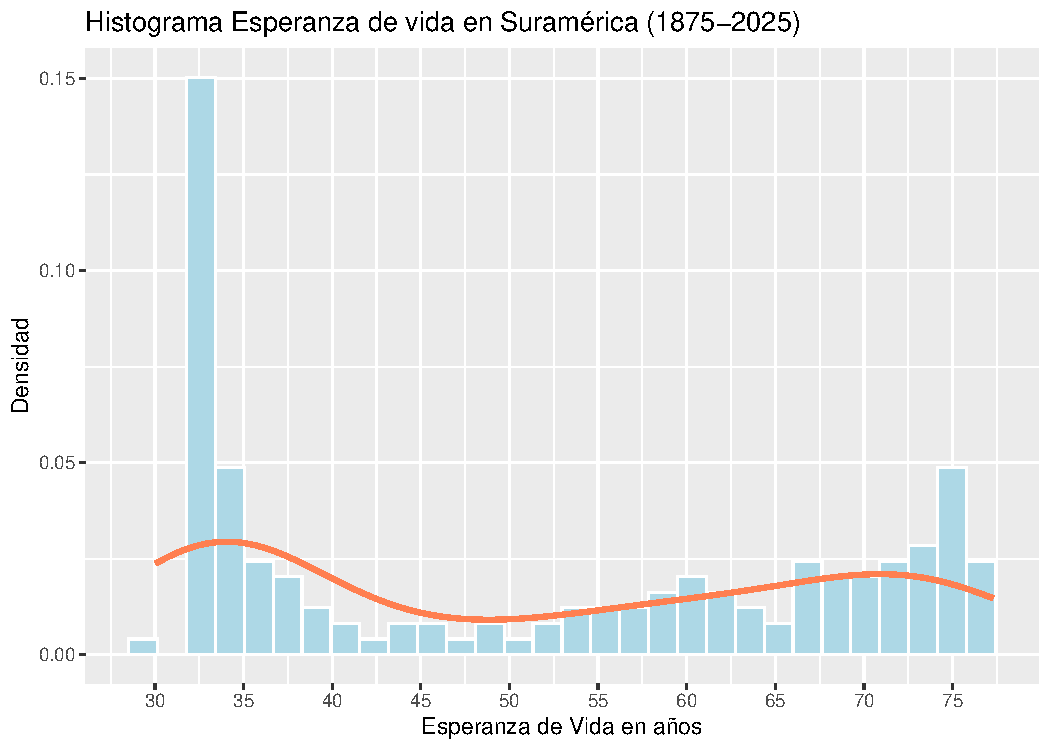
\includegraphics{presentacion_Parada_G_M8R2-002}
\end{frame}


\begin{frame}[fragile]
\frametitle{Análisis del histograma}
\begin{itemize}
\item<1> Al observar la distribución de densidad de la Esperanza de Vida de los países de Suramérica en los últimos 150 años se nota que un tercio de la misma se situa entre los 30 y 37.5 años.
\item<2> Luego incrementa rápidamente y se estabiliza un poco entre el rango de 70 a 80 años.
\end{itemize}
\end{frame}


% Diapositiva gráfico de líneas Esperanza de vida por países
\begin{frame}{fragile}
\frametitle{Esperanza de vida por país}
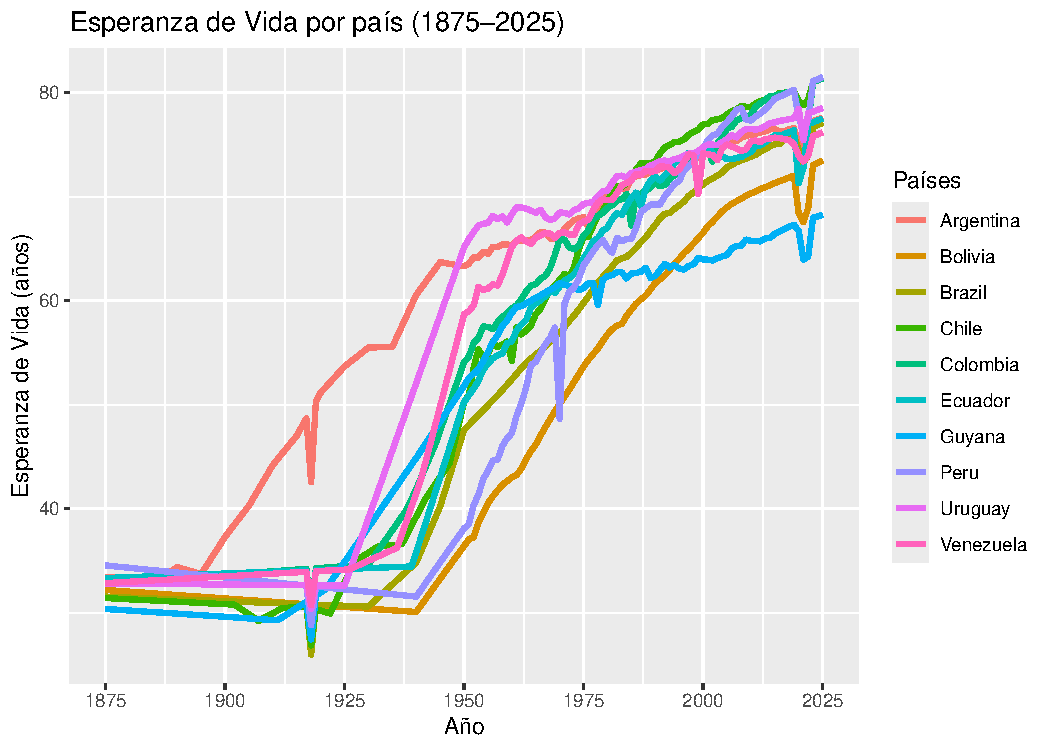
\includegraphics{presentacion_Parada_G_M8R2-003}
\end{frame}


% Diapositiva explicación del gráfico de líneas
\begin{frame}[fragile]
\frametitle{Esperanza de vida por país}
\begin{itemize}
\item<1> Entre 1925 y 1935 se observa un rápido incremento en la Esperanza de Vida.
\item<2> Bolivia y Guyana se han quedado rezagados en el aumento de la Esperanza de Vida. Guyana es un caso interesante porque en los últimos años ha tenido un crecimiento económico acelerado, pero esto no se ha reflejado por los momentos en una mejora de la Esperanza de Vida.
\item<3> Argentina es un outlier gozando de un incremento de la Esperanza de Vida desde 1890. Algunas de las razones fueron: Un crecimiento económico temprano, urbanización controlada y políticas de salud pública pioneras hicieron que cayera de forma drástica la mortalidad infantil.
\end{itemize}
\end{frame}


% Diapositiva gráfico de líneas GDP per cápita PPP por país (1875–2025)
\begin{frame}{fragile}
\frametitle{GDP per cápita PPP por país}
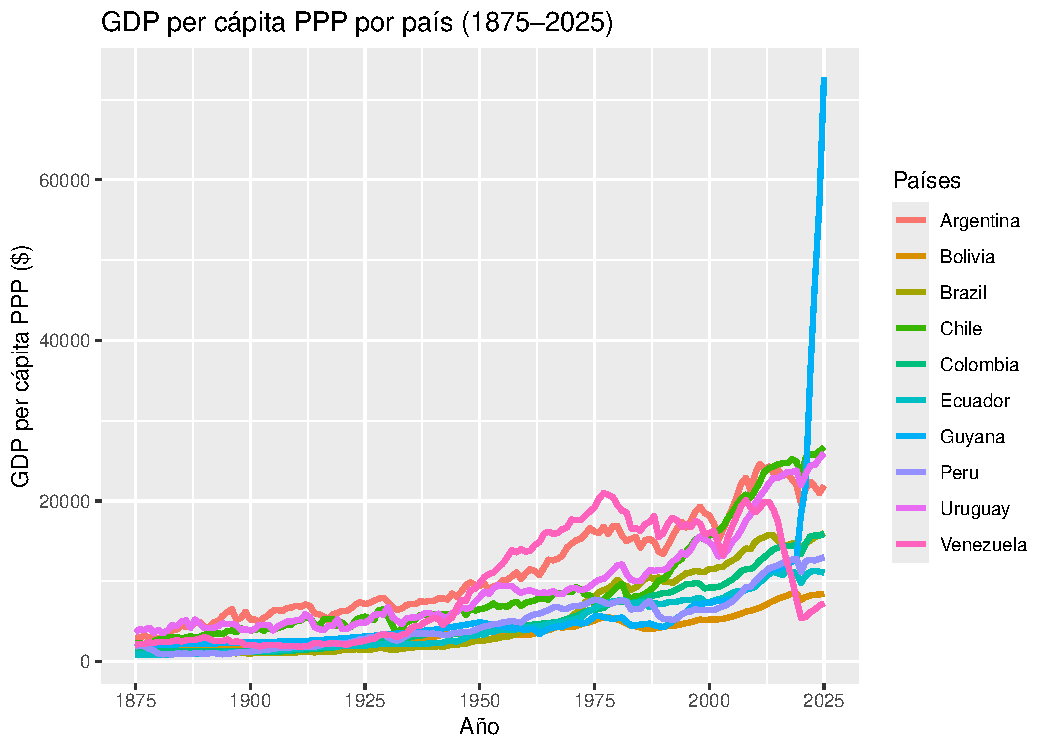
\includegraphics{presentacion_Parada_G_M8R2-004}
\end{frame}

% Diapositiva explicación gráfico de líneas GDP per cápita PPP por país (1875–2025)
\begin{frame}[fragile]
\frametitle{GDP per cápita PPP por país}
\begin{itemize}
\item<1> La tendencia general es que todos los países de Suramérica han aumentado su GDP per cápita PPP.
\item<2> Venezuela en terminos de GDP per cápita PPP fué entre los años 1950 y finales de la década de 1990 el país con mayor poder adquisitivo. Seguido por una grave crisis económica a inicios de la década del 2010.
\item<3> Guyana ha sido históricamente un país con un bajo GDP Per cápita PPP, pero en 2015 se descubrieron grandes pozos petroleros en sus costas. En el año 2019 empezó la explotación lo que ha aumentado su GDP per cápita PPP de 12800\$ en ese año hasta 72800\$ en el 2025 y se espera que continue este crecimiento económico.
\end{itemize}
\end{frame}


% Diapositiva de gráfico de correlación entre GDP  PPP y Esperanza de Vida
\begin{frame}{fragile}
\frametitle{Correlación entre GDP  PPP y Esperanza de Vida Suramérica (1875-2025)}
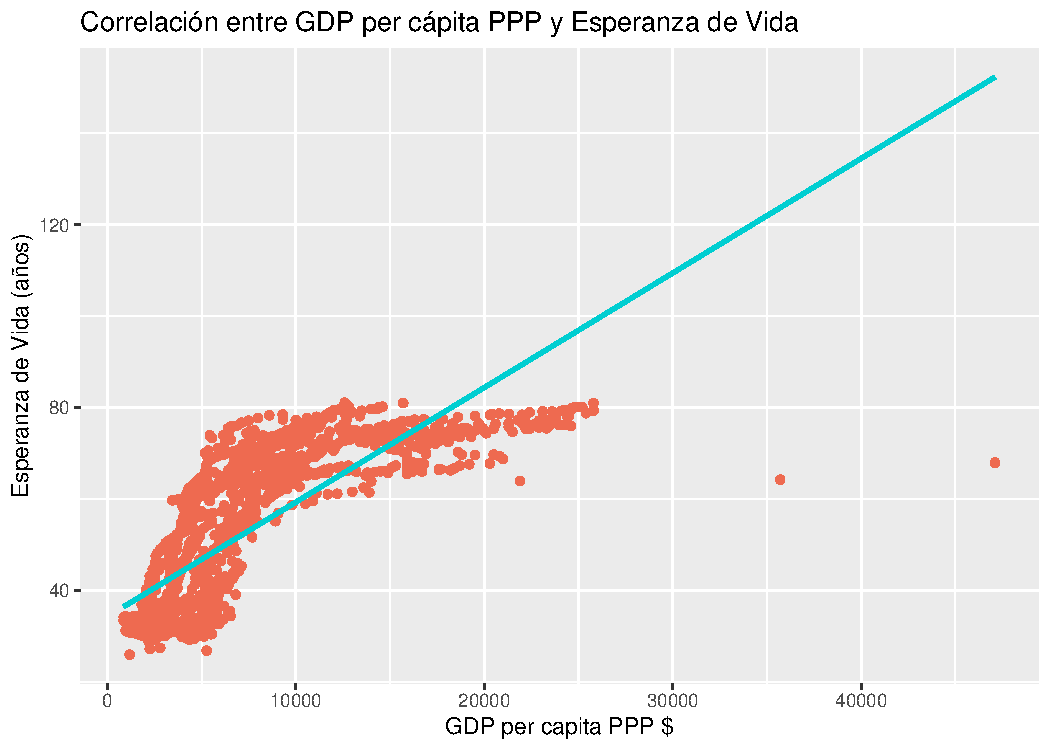
\includegraphics{presentacion_Parada_G_M8R2-005}
\end{frame}


% Diapositivas análisis de gráfico de correlación
\begin{frame}[fragile]
\frametitle{Correlación entre GDP PPP y Esperanza de Vida Suramérica (1875-2025)}
\begin{itemize}
\item<1> Se observa una correlación positiva y fuerte entre el GDP per cápita PPP y la Esperanza de Vida de un país.

\item<2> El coeficiente de correlación de Pearson de ambas variables para Suramérica es de: 0.76.

\item<3> Aunque es fuerte y positivo, hay otras variables socio-económicas y ambientales que influyen en la Esperanza de Vida. Por ejemplo, el acceso a la sanidad pública, estilos de vida, nivel educativo.

\item<4> Por lo que a pesar de las condiciones económicas, es importante tomar responsabilidad en salud preventiva.
\end{itemize}
\end{frame}


% Diapositiva de Referencias
\begin{frame}[fragile]
\frametitle{Referencias}
{\scriptsize
- Gapminder Foundation. (2023). Life expectancy at birth (Documentation, version 14) [Dataset]. Gapminder. https://www.gapminder.org/data/documentation/gd004/

- Gapminder Foundation. (2025). GDP per capita in constant PPP dollars (documentation, version 31, PPP2021) [Dataset]. Gapminder. https://www.gapminder.org/data/documentation/gd001/

- Mee, A. (2023, 11 de diciembre). Guyana: Del "boom" petrolero al riesgo de la "maldición de los recursos". Global Affairs and Strategic Studies, Universidad de Navarra. https://www.unav.edu/web/global-affairs/guyana-del-boom-petrolero-al-riesgo-de-la-maldicion-de-los-recursos

- Lodeiro, A. R. (2020). Esperanza de vida al nacer. Contribuciones y desafíos de la microbiología. Revista Argentina de Microbiología, 52 (2), 85–87. Asociación Argentina de Microbiología. https://doi.org/10.1016/j.ram.2020.03.001

- Astorga, P. (2003). La economía venezolana en el siglo XX. Revista de Historia Económica, Año XXI, 623–653. Universidad Carlos III de Madrid. https://e-archivo.uc3m.es/rest/api/core/bitstreams/64513b90-8f71-4cfe-bcd4-6f7e2d8653fb/content
}

\end{frame}
\end{document}
